\documentclass{article}
\title{Nechyba Ch.23 垄断}
\author{Dawei Wang}
\date{\today}
\usepackage{ctex}
\usepackage{amsmath}
\usepackage{amssymb}
\usepackage{graphicx} %插入图片的宏包
\usepackage{float} %设置图片浮动位置的宏包
\usepackage{subfigure} %插入多图时用子图显示的宏包
\begin{document}
	\maketitle
垄断厂商拥有一些竞争性厂商不具有的相对试产(即价格)的控制权。

垄断势力是源于某种程度的集中性。在完全竞争市场中,由于有很多厂商都会在市场给定的价格下生产相同的产品,所以每个厂商面临的需求曲线都是具有完全弹性的。那么不论何时,只要一个厂商所面临的产品需求曲线不是具有完全弹性的,该厂商就具有一定的市场势力。

在某些前提下,特定厂商所生产的产品的替代品并不容易获得。假设市场壁垒存在并阻止潜在竞争者去生产替代品,此时我的市场垄断势力将变得更为显著,而我的产品所面临的需求也将变得更加没有弹性。垄断产品需求弹性的大小和其垄断势力的强弱紧密相关。

\section{垄断者的定价决策}
\subsection{需求、边际收益与利润}

对于完全竞争厂商来说,销售价格等于边际收益。因此尽管在完全竞争市场中市场需求曲线是向右下方倾斜的,但在确定的市场价格下单个完全竞争厂商面临的需求曲线都是具有完全弹性的。

由于垄断市场中只有一个厂商,所以对于一个垄断市场来说,市场需求就是厂商需求。当一个垄断厂商决定提高产量时,它将面临以下权衡:一方面,它将向消费者出售更多的产品;另一方面,它必须以低于之前价格的价格出售其全部产品。因此,当垄断厂商增加产出时,其边际收益就不再与开始索取的价格相等了,这是因为想要卖掉这些增加的额外产品它必须降低价格。

\begin{figure}[H] %H为当前位置,!htb为忽略美学标准,htbp为浮动图形
	\centering %图片居中
	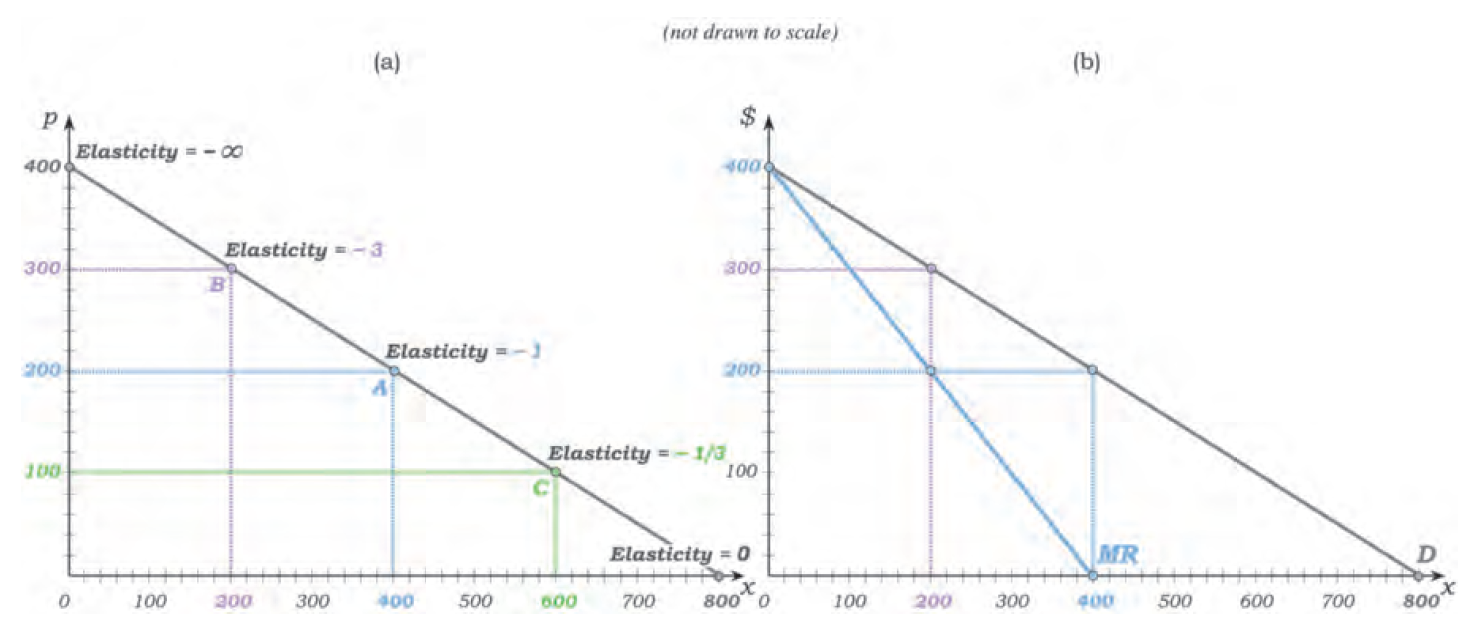
\includegraphics[width=1\textwidth]{23_1} %插入图片,[]中设置图片大小,{}中是图片文件名
	\caption{Linear Demand and Marginal Revenue} %最终文档中希望显示的图片标题
	\label{Fig.main2} %用于文内引用的标签
\end{figure}

\hspace*{\fill}

需求价格弹性与收益最大化

当价格弹性低于-1时边际收益为正;当需求弹性接近-1时,边际收益接近零。

当需求缺乏弹性时,价格上升消费者支出也随之上升,反之反是。一方面,当垄断厂商发现消费者对自己的产品需求缺乏弹性时,它知道提价收益就会增加;另一方面,当垄断厂商发现对自己的产品需求富有弹性时,它可以通过降价来使收益增加。

\begin{figure}[H] %H为当前位置,!htb为忽略美学标准,htbp为浮动图形
	\centering %图片居中
	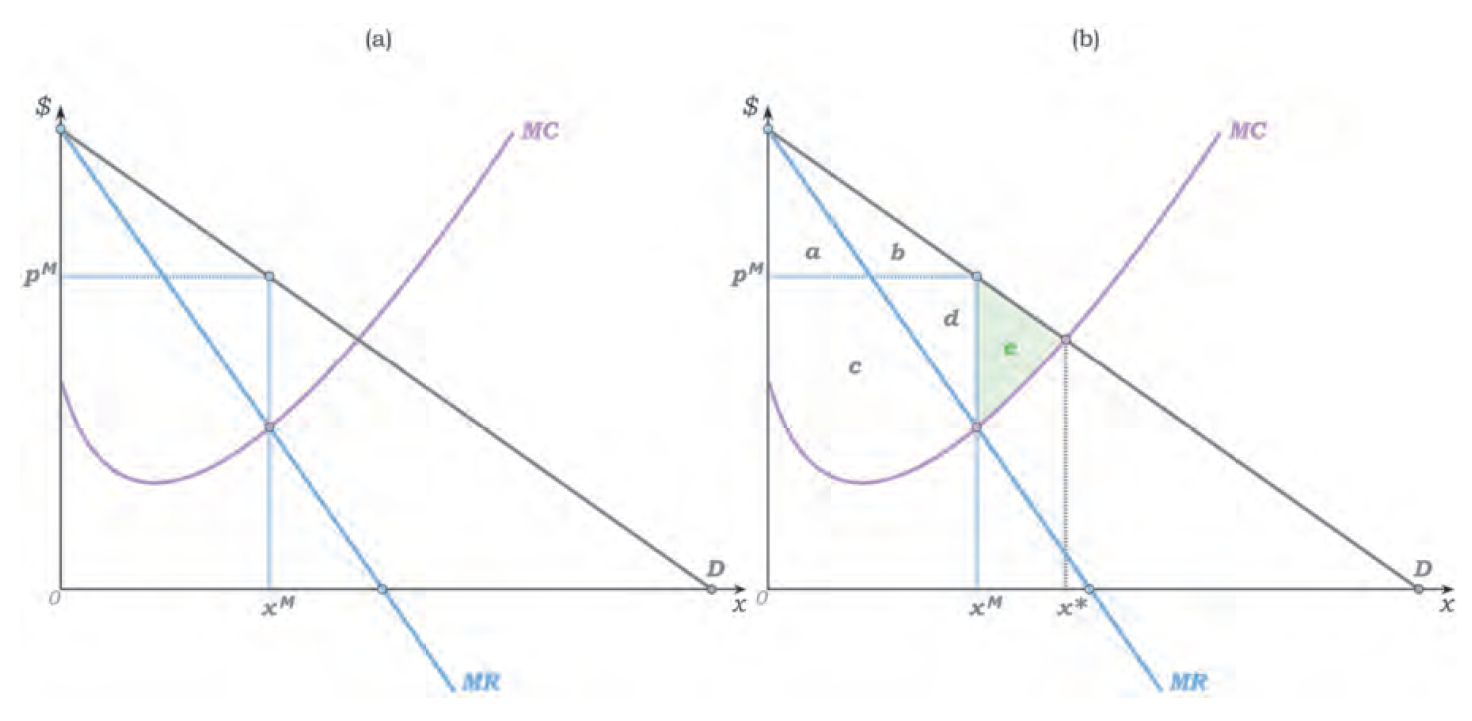
\includegraphics[width=1\textwidth]{23_2} %插入图片,[]中设置图片大小,{}中是图片文件名
	\caption{Profit Maximization for a Monopolist} %最终文档中希望显示的图片标题
	\label{Fig.main3} %用于文内引用的标签
\end{figure}

只要MC是正的,垄断厂商就会选择在需求曲线富有弹性的部分进行生产。这是因为任何正的MC,MC和MR的交点必定位于MR与水平轴交点的左方。如果垄断厂商发现自己处于需求无弹性范围内,它将可以通过减少产量提高价格,同时提高收益和降低成本。因此,垄断厂商在需求无弹性范围内生产是没有意义的。

\hspace*{\fill}

垄断厂商不存在供给曲线。供给曲线描述了由市场给定的价格与由厂商利润最大化决定的产量之间的关系,但是垄断厂商没有“市场”来给定价格,而是垄断厂商自己确定价格。因此,对于任何给定的需求曲线与任何方法推导出的成本曲线,垄断厂选择的仅仅是一些供给点(supply point)。

\hspace*{\fill}

竞争条件下:给定信号:市价$\rightarrow\max\limits_{\pi}\rightarrow$产出——供给曲线,价格外生;

垄断:需求曲线$\rightarrow\max\limits_{\pi}\rightarrow$(产出,价格)——供给点,价格内生。

\hspace*{\fill}

对于超出厂商决定供给的那一部分,厂商依然还有能力来生产额外的一部分产品,对于这部分产品其边际成本高于消费者愿意支付的价格,这部分额外产出可以一直增加到MC曲线与需求曲线相交的产量$ x^* $处,即如果生产是由一位社会规划者来制定而不是一个垄断组织来决定,那么消费者剩余将会增加(e)部分。因此面积(e)是无谓损失,其源于垄断者的利润最大化而策略性地限制产出(或来源于其垄断地位)。

无谓损失的出现并不是因为垄断厂商获得了利润。即使垄断者被强制生产$ x^* $,它还是可以获得利润,只是利润不如不受限制时那么大。垄断者的市场势力引起了自身利益与社会福利的冲突——至少当社会福利是效率的评价标准时——除非某种力量进行干预使垄断厂商增加产量。

垄断者的寻租行为与无谓损失

如果厂商通过某种方式获得了一些垄断势力,它们就能够获得经济利润。这种经济利润会造成社会成本,因为垄断厂商为了使价格超过边际成本其产出水平将低于社会最优产出水平,这种社会成本被称为无谓损失。然而实际的无谓损失可能远远超过现在推导的内容,因为厂商为了获得和维持垄断地位从而获得垄断利润,其可能会进行一些无任何意义的社会活动。

厂商为了得到政府赋予的垄断势力而愿意支付的最大费用等于未来厂商可以利用这种垄断势力得到的垄断利润的现值。这就是政治寻租。

\subsection{市场分割与价格歧视}

至今为止的结果都建立在垄断厂商不能有效区分消费者类型并发现其边际支付意愿的情况下,或在对不同类型价格消费者索取不同价格是违法的情况下是正确的。在本节中,假设对不同的消费者索取不同价格,即允许价格歧视(price discrimination),并且垄断者可以把消费者分成两部分:一部分愿意支付相对较高的价格,另一部分愿意支付相对较低的价格。不过,即使垄断者可以根据不同的消费者划分出不同的市场类型,它也必须要有办法来阻止二次销售,即阻止以低价购买的消费者把商品出售给本需以高价购买的消费者行为。

\hspace*{\fill}

价格歧视的三种形式:

一级价格歧视:

垄断者可以完全确定每个消费者的需求,并可以以特定的价格为每个消费者提供特定数量的产品。达到这种目的的一个方式是,向每个消费者索取能够获得购买权的固定费用和为购买每单位商品所支付的费用,并且针对不同的消费者,固定费用和产品单价也都不相同/这就是完全(“一级”)价格歧视。

三级价格歧视:

垄断厂商依然能够完全区分每个消费者的需求并可以向每个想消费多单位商品的不同消费者索取不同的单位商品价格(但是没有固定费用)。

二级价格歧视:

垄断者知道存在具有不同消费需求的不同类型消费者,但是它不知道每个特定的消费者属于哪种类型。因此垄断厂商设置了价格/数量组合,或固定费用与单位产品价格的组合,使消费者自己去“揭示他们的消费类型”。

\hspace*{\fill}

完全(一级)价格歧视:

\begin{figure}[H] %H为当前位置,!htb为忽略美学标准,htbp为浮动图形
	\centering %图片居中
	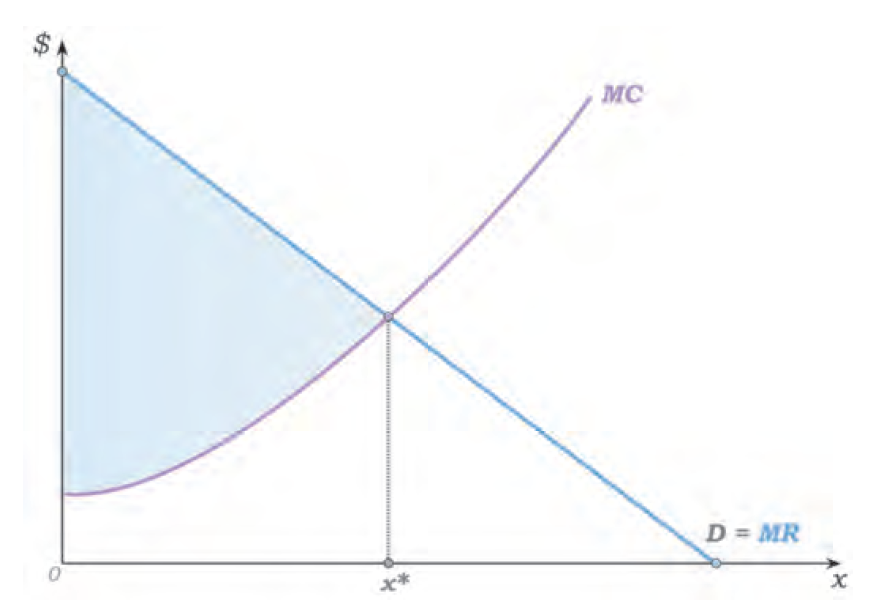
\includegraphics[width=1\textwidth]{23_3} %插入图片,[]中设置图片大小,{}中是图片文件名
	\caption{Perfect Price Discrimination} %最终文档中希望显示的图片标题
	\label{Fig.main4} %用于文内引用的标签
\end{figure}

此时需求等于MR,生产者选择MC曲线与需求曲线的交点$ x^M $的产量水平。消费者剩余为零,所有的剩余,即阴影部分,都属于垄断厂商。在这个过程中,厂商达到了有效的产量水平,任何额外产出的成本都将超过其社会价值。

当消费者购买多单位产品,并且被索取他们为每单位产品愿意支付的价格时,这种完全价格歧视的形式也被称为一级价格歧视。

不完全或“三级”价格歧视

\begin{figure}[H] %H为当前位置,!htb为忽略美学标准,htbp为浮动图形
	\centering %图片居中
	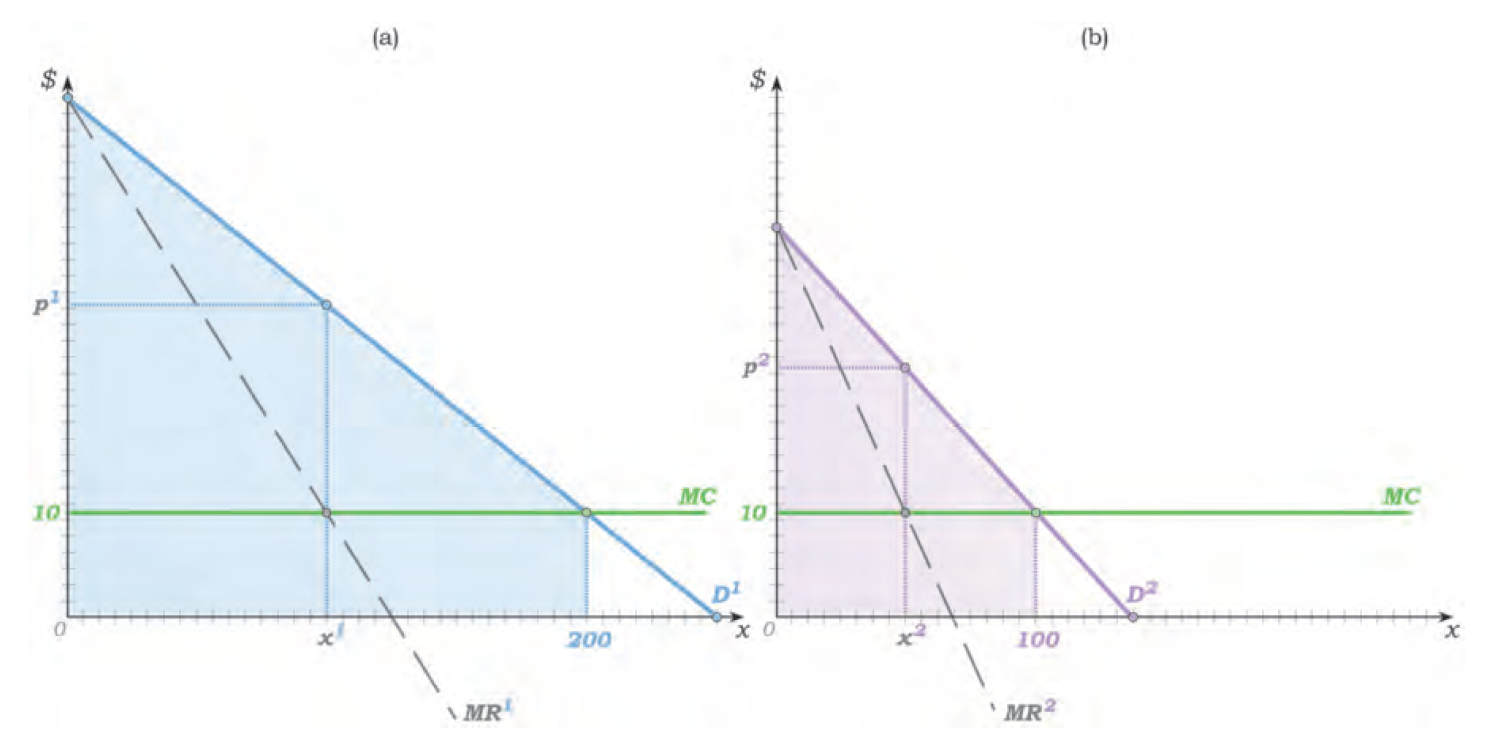
\includegraphics[width=1\textwidth]{23_4} %插入图片,[]中设置图片大小,{}中是图片文件名
	\caption{Imperfect (“Third Degree”) Price Discrimination} %最终文档中希望显示的图片标题
	\label{Fig.main5} %用于文内引用的标签
\end{figure}

可以区分不同消费者类型的垄断厂商对商品只能收取一个价格,这个价格对不同的消费者类型是不同的,但是购买数量在某个范围内的消费者被索取的价格都是相同的。如果是这样,垄断厂商就不能实施完全价格歧视,只能实施不完全价格歧视了,这种价格歧视也被称为“三级价格歧视”。

当厂商对可以区分的不同类型的消费者索取不同的产品单价时,它们将会把产量限制在低于完全价格歧视时的有效的产量水平。结果就是,不完全价格歧视会导致无谓损失。

尽管知道三级价格歧视将会导致无谓损失,但是如果消除垄断厂商这种价格歧视的定价能力,无谓损失变小还是变大,这一点我们并不清楚。我们需要在低需求消费者的福利损失加上垄断厂商的利润减少与高需求消费者得到的福利增加之间相权衡。三级价格歧视的取消可能会使总体福利增加(如果高需求消费者的福利增加超过低需求消费者和垄断厂商的福利减少),也可能会使总体福利减少(如果低需求消费者和垄断厂商的福利损失超过高需求消费者的福利增加)。

\hspace*{\fill}

非线性定价与“二级价格歧视”

有时候厂商可以利用外部信号区分它所面临的消费者类型。但是现实生活中,厂商可能没有这样的信号可以利用,因此也就不能随时确定它所面临的消费者属于哪种类型。

由于垄断厂商不能分辨它所面临的消费者属于何种类型,它不得不以某种方式设置价格,给消费者一些激励使他们自我分组。这涉及单一非线性定价策略的设定,或者给不同数量的产品制定不同的价格。

\subsection{进入壁垒与对无效垄断行为的补救}

垄断厂商为了赚得长期正的利润,对新厂商必须制造一些进入壁垒。这些壁垒的出现可能是由于生产技术的自然属性,也可能是由于不同类型的合法限制。

\hspace*{\fill}

进入的技术壁垒与自然垄断

现假定对商品X的生产过程一直都是规模报酬递增的,这意味着MC曲线一直都是向下倾斜的,并且一直位于AC曲线的下方这又意味着任何一个完全竞争的厂商在价格给定的情况下有可能一点都不生产,也有可能生产无限数量的产品。但是,在资源稀缺的现实世界中,消费者对于有着正的价格的商品的需求不可能是无穷的,也就是说在规模报酬递增的情况下厂商的价格接受行为假设并不合理。

自然垄断(natural monopoly)厂商被定义为全部产出数量水平上其AC曲线一直向下倾斜的厂商。该向下倾斜的AC曲线可能是由于规模报酬递增引起的,或者是由于反复出现的固定成本与不变边际成本引起的。无论是哪种情况,我们都不能找出一条MC曲线位于AC曲线上方的“供给曲线”,因为MC曲线不可能超过AC曲线。因而这样一个厂商很自然地成为了一个垄断厂商。

\begin{figure}[H] %H为当前位置,!htb为忽略美学标准,htbp为浮动图形
	\centering %图片居中
	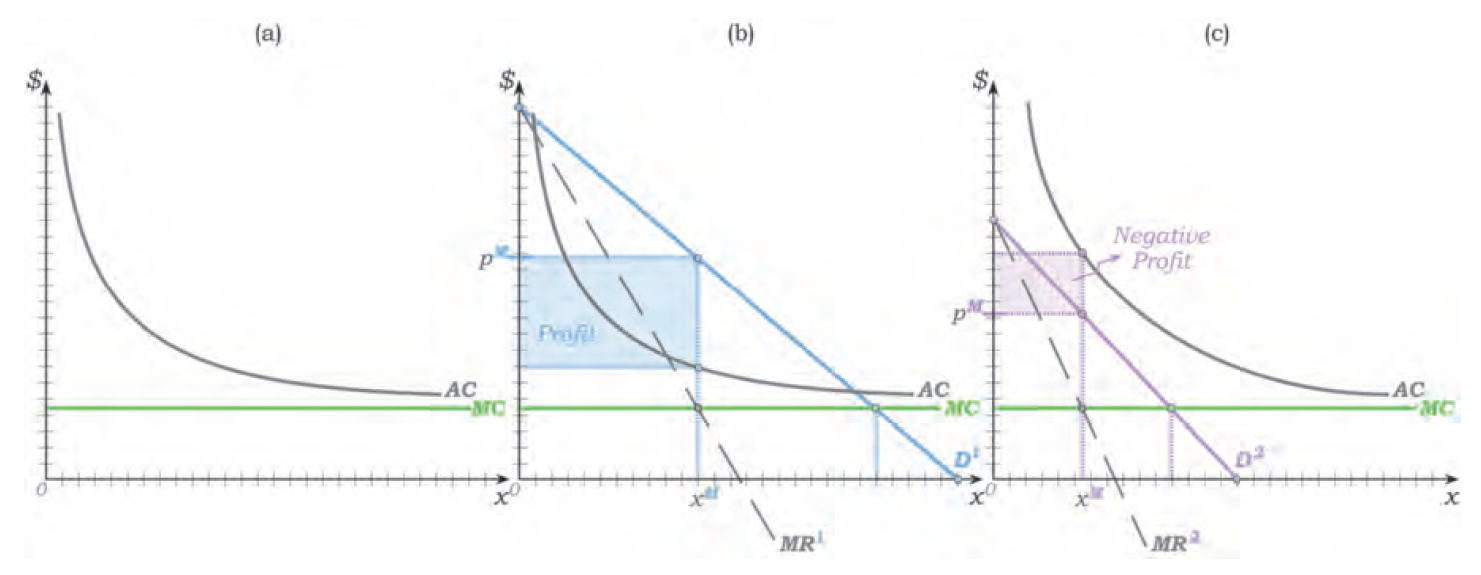
\includegraphics[width=1\textwidth]{23_5} %插入图片,[]中设置图片大小,{}中是图片文件名
	\caption{Imperfect (“A Natural Monopoly”) Price Discrimination} %最终文档中希望显示的图片标题
	\label{Fig.main6} %用于文内引用的标签
\end{figure}

一旦垄断厂商开始运作,固定成本即变成沉淀成本,所以有效的产出水平应该出现在MC曲线与需求曲线地交点处。

假设垄断厂商面临着较高的反复出现的固定成本。那么试图使自然垄断厂商达到有效率产出水平的管制者可能会通过MC曲线定制价格为目标,并允许垄断厂商向消费者额外索取一个独立于消费水平的“固定费用”。自然垄断厂商为了得到更多的固定费用补贴以及更高的单位价格,它有很强烈的动机向管制者放大其成本。即使垄断厂商会很诚实地说出实际发生的成本规模,它也没有特别的动机去进行一些能减少成本的研发创新。

\hspace*{\fill}

合法的进入壁垒

合法的进入壁垒可能来源于普通专利和版权的法律保护,它赋予那些有专利和版权的公司生产特定产品的排他性权利。如果厂商能够成功地游说政府来保护来自竞争者的攻击,并且这种游说所需的成本小于合法壁垒形成后所得的垄断利润的现值,那么厂商就会花费资源努力达到游说目标。这种游说是纯粹的社会浪费活动,政府建立的垄断引起的无谓损失可能会超过在垄断利润最大化动机驱使下的产量减少引起的损失。


\hspace*{\fill}

限制垄断势力

创新专利保护使得一些产品的出现成为可能,这就意味着社会剩余的增加,尽管如果强制垄断厂商生产更多会带来更多的社会剩余。由于管制者并不知道厂商的真实成本,并且这些管制将会降低垄断厂商进行创新的积极性,所以直接对垄断厂商定价进行管制会有信息限制。因此管制并不是所有情况下的万能药。

\section{垄断的数学分析}

被限制只能设定单一价格的垄断者需要解决的问题:

\[
\max\limits_{x,p}\pi=px-c(x)\enspace and\enspace p\le p(x)
\]

垄断厂商在试图出售x数量产品时所收取的价格不能超过反需求函数p(x)上对应产量点的价格。

既然垄断厂商会把价格尽可能地提高至可以卖出其所生产地所有产品的水平,那么不等式$ p\le p(x) $将被限制为$ p=p(x) $。那么垄断厂商的最优化问题就可以表示为:

\[
\max\limits_{x} \pi=p(x)x-c(x)
\]

一旦我们将约束条件代入最优化问题中的目标函数,垄断厂商选择最优产量$ x^M $,也就隐含选择了最优价格$ p^M=p(x^M) $。由于产量与价格的一一对应关系,垄断厂商的最优化问题也可以表示为:

\[
\max\limits_{p} \pi=px(p)-c(x(p))
\]

如果厂商可以在消费者进行消费选择前分清消费者类型,一级和三级价格歧视就可行(假设转售可以被制止);如果厂商只知道每个类型的消费者的数量分布,二级价格歧视就可行。这些不同形式的价格歧视会受到公司所允许的定价策略的进一步限制,然而从根本上讲,厂商依然只是通过制定产量决策和采用差别定价策略来使利润最大化。

需求、边际收益与利润

\begin{equation*}
	\begin{split}
	MR&=p(x)+\frac{dp}{dx}x\\
	&=p(x)(1+\frac{dp}{dx}\frac{x}{p(x)})\\
	&=p(x)(1+\frac{1}{\epsilon_D})
	\end{split}
\end{equation*}

\hspace*{\fill}

利润最大化:

\[
MR=p(x)+\frac{dp}{dx}x=MC
\]

\hspace*{\fill}

垄断加成(monopoly markup ratio)/勒纳指数(Lerner Index)

\[
\frac{p-MC}{p}=\frac{-1}{\epsilon_D}
\]

价格与边际成本之间的差额(即p-MC)被称为垄断加成(monopoly markup)。勒纳指数(价格加成率)反应了厂商的垄断程度。当价格弹性趋于负无穷大时,垄断加成率趋于0,垄断厂商面临的需求曲线也越来越类似于完全竞争厂商所面临的需求曲线。

\hspace*{\fill}

\subsection{当消费者类型可区分时的价格歧视
}

完全或一级价格歧视

对于一级价格歧视的一种实现形式即两部收费制,消费者唯一的问题就是他是否愿意为了从垄断厂商那里获得购买权力而支付这笔固定费用。既然当没有固定费用时只有单一产品价格时消费者有$ CS^n $部分的剩余,那么当固定费用小于等于$ CS^n $时消费者就愿意支付这笔固定费用。因此垄断厂商可以设置两部收费制,即对消费者n索取的总支付$ P^n $等于

\[
p^n(x)=CS^n+p^cx
\]

在两部收费制下,垄断厂商可以为消费者n制定一个价格,是的消费者剩余变为零,但会达到有效的消费量水平。对于每种不同类型的消费者的固定费用也都是不同的,这意味着如果消费者有着不同的需求,垄断厂商为了实施一级价格歧视必须知道每个消费者的需求类型。

\[
MR^1=MC=MR^2
\]

\[
p^1(1+\frac{1}{\epsilon_D^1})=MC=p^2(1+\frac{1}{\epsilon_D^2})
\]

\subsection{当消费者类型不可区分时的价格歧视
}

单一两部收费制的二级价格歧视
















































































\end{document}